\documentclass[11pt,a4paper]{article}

% Required base packages
\usepackage{graphicx}
\usepackage{xcolor}
\usepackage{geometry}
\usepackage{amsmath}
\usepackage{amssymb}
\usepackage{booktabs}
\usepackage{longtable}
\usepackage{array}
\usepackage{colortbl}
\usepackage{enumitem}
\usepackage{tcolorbox}
\usepackage{fancyhdr}
\usepackage{titlesec}
\usepackage{tocloft}
\usepackage{setspace}
\usepackage{microtype}
\usepackage{parskip}
\usepackage{marginnote}
\usepackage{multicol}
\usepackage{float}
\usepackage{wrapfig}
\usepackage{tikz}
\usepackage{caption}
\usepackage{subcaption}
\usepackage{afterpage}
\usepackage{pdfpages}
\usetikzlibrary{shapes,arrows,positioning,calc}

% Page geometry
\geometry{a4paper, top=2.5cm, bottom=2.5cm, left=2.5cm, right=2.5cm}

% Colors
\definecolor{darkblue}{RGB}{0,51,102}
\definecolor{burgundy}{RGB}{128,0,32}
\definecolor{gold}{RGB}{184,134,11}
\definecolor{lightgray}{RGB}{245,245,245}
\definecolor{darkgray}{RGB}{64,64,64}
\definecolor{newspaperbg}{RGB}{255,250,240}

% hyperref - MUST load last
\usepackage[
    colorlinks=true,
    linkcolor=darkblue,
    citecolor=darkgray,
    urlcolor=darkblue,
    bookmarks=true,
    bookmarksnumbered=true,
    unicode=true,
    pdftitle={The Buckler Family Case: A Path to Justice},
    pdfauthor={Buckler Family Research},
    pdfsubject={Historical Land Injustice and Legal Remedies},
    pdfkeywords={BP vs Buckler, Great House Farm, Land Justice, Wales}
]{hyperref}

% Header/Footer setup
\pagestyle{fancy}
\fancyhf{}
\fancyhead[L]{\small\textcolor{darkgray}{The Buckler Family Case}}
\fancyhead[R]{\small\textcolor{darkgray}{\leftmark}}
\fancyfoot[C]{\thepage}
\renewcommand{\headrulewidth}{0.4pt}

% Section formatting
\titleformat{\section}{\Large\bfseries\color{darkblue}}{\thesection}{1em}{}
\titleformat{\subsection}{\large\bfseries\color{burgundy}}{\thesubsection}{1em}{}
\titleformat{\subsubsection}{\normalsize\bfseries\color{darkgray}}{\thesubsubsection}{1em}{}

% tcolorbox styles
\tcbuselibrary{skins,breakable}

\newtcolorbox{keyfact}{
    colback=lightgray,
    colframe=darkblue,
    fonttitle=\bfseries,
    title=Key Fact,
    breakable
}

\newtcolorbox{grievance}{
    colback=red!5,
    colframe=burgundy,
    fonttitle=\bfseries,
    title=Grievance,
    breakable
}

\newtcolorbox{action}{
    colback=green!5,
    colframe=green!50!black,
    fonttitle=\bfseries,
    title=Action Item,
    breakable
}

\newtcolorbox{timeline}{
    colback=gold!10,
    colframe=gold!70!black,
    fonttitle=\bfseries,
    title=Timeline Entry,
    breakable
}

\newtcolorbox{newspaperquote}{
    colback=newspaperbg,
    colframe=darkgray,
    fonttitle=\bfseries\itshape,
    title=Newspaper Report,
    breakable
}

% Line spacing
\setstretch{1.15}

\begin{document}

% Title Page
\begin{titlepage}
\centering
\vspace*{2cm}

{\Huge\bfseries\color{darkblue} THE BUCKLER FAMILY CASE}\\[0.5cm]
{\LARGE\color{burgundy} A Quest for Justice}\\[1cm]

\rule{\textwidth}{1.5pt}\\[0.5cm]
{\Large\bfseries BP Properties Ltd v Buckler (1987)\\
Great House Farm, Llandough, Wales}\\[0.5cm]
\rule{\textwidth}{1.5pt}\\[2cm]

{\large\itshape ``It's my land. It's not your permission to give.''}\\[0.3cm]
{\normalsize --- Mary Williams Buckler, October 1974}\\[2cm]

\begin{tcolorbox}[colback=lightgray,colframe=darkblue,width=0.9\textwidth]
\centering
\textbf{A Comprehensive Documentation of Historical Land Injustice,\\Legal Analysis, and Strategic Roadmap to Justice and Compensation}

\vspace{0.5cm}
\textit{With Original Newspaper Archive Evidence}
\end{tcolorbox}

\vfill

{\large Document compiled: January 2026}\\[0.5cm]
{\normalsize For the Buckler Family and Future Generations}

\end{titlepage}

% Table of Contents
\tableofcontents
\newpage

% Executive Summary
\section{Executive Summary}

This document presents a comprehensive analysis of the Buckler family's historical land dispute involving Great House Farm at Llandough, near Penarth, Wales. The case culminated in the landmark legal decision \textit{BP Properties Ltd v Buckler} (1987), which resulted in the displacement of a family that had occupied the land for over 400 years.

\begin{keyfact}
The Buckler family (previously Williams) occupied Great House Farm, Llandough, since the 1600s --- approximately 400 years of continuous occupation. The family was physically removed after the 1987 legal case, and the 800-year-old farm was subsequently demolished.
\end{keyfact}

\subsection{Core Allegations}

The Buckler family maintains they were subjected to:

\begin{enumerate}[label=\arabic*.]
    \item \textbf{Historical Land Theft}: The systematic dispossession of their ancestral farm through legal mechanisms that favored corporate interests over occupiers' rights.
    \item \textbf{Procedural Unfairness}: Courts that allegedly favored ground rent interests over the family's historic tenancy context and hardship circumstances.
    \item \textbf{Abuse of Process}: Civil mechanisms used coercively without adequate criminal basis, including the use of detention to clear land.
    \item \textbf{Unjust Enrichment}: Corporate beneficiaries (BP and successors) retaining gains from forced clearance.
    \item \textbf{Historical Erasure}: The possible suppression of the family's connection to significant historical events, including Marconi's radio experiments.
\end{enumerate}

\subsection{The Marconi Connection}

A significant but under-explored aspect of this case involves Guglielmo Marconi, the inventor of radio. Historical accounts indicate that:

\begin{timeline}
In May 1897, at age 22, Guglielmo Marconi stayed at Great House Farm while conducting his wireless telegraphy experiments. The Williams family (Buckler ancestors) reportedly transported Marconi and his equipment by horse and cart to Lavernock Point for his historic first radio transmission over open sea.
\end{timeline}

The family's claim that a dining table used by Marconi during his experiments was sold in the 1970s adds a material dimension to this connection. The absence of any commemoration or acknowledgment of this historical fact in the local area raises questions about historical erasure.

\subsection{Current Status}

The Buckler family continues to seek:
\begin{itemize}
    \item Justice for the loss of their home, livelihood, and heritage
    \item Financial compensation for unlawful dispossession
    \item Public recognition of the historical injustices committed
    \item Correction of historical records
    \item Return of any archaeological treasures excavated from beneath the farm (1994)
\end{itemize}

\newpage

% Historical Background
\section{Historical Background}

\subsection{Ancient Origins of the Site}

Great House Farm, Llandough, occupies a site of extraordinary historical significance dating back over 1,500 years.

\subsubsection{Early Medieval Period (6th--11th Century)}

\begin{timeline}
\textbf{525 A.D.} --- The Council of Clermont divided diocesan clergy into categories, establishing frameworks for rural churches and estate chapels. The religious community at Llandough was well-established by the 6th century.
\end{timeline}

The site of Great House Farm overlay one of the major early-medieval monasteries of Glamorgan. Archaeological evidence from the 1994 excavation revealed:

\begin{itemize}
    \item A post-Roman cemetery with over 1,000 burials
    \item Evidence of continuous occupation from the late Iron Age
    \item A 6th--10th century monastic community dedicated to Saint Dochdwy
    \item The largest early Christian cemetery excavated in Wales
\end{itemize}

\subsubsection{Roman Period (2nd--4th Century)}

\begin{timeline}
\textbf{2nd Century A.D.} --- A Roman villa was constructed on the site, which developed considerably in the early 3rd century and remained occupied until the early 4th century.
\end{timeline}

The villa was substantial, containing at least five rooms with a hypocaust system, and compared in size and status with those at Llantwit Major and Ely.

\subsubsection{Medieval Grange (12th--16th Century)}

\begin{timeline}
\textbf{11th Century} --- The village of Llandough was granted to Tewkesbury Abbey, and a grange was subsequently established. This remained in Tewkesbury's ownership until the Dissolution when it was confiscated by the Crown.
\end{timeline}

Archaeological evidence recovered included:
\begin{itemize}
    \item A dovecote and barn possibly dating to the late 12th century
    \item Walls of the Roman villa reused as foundations for medieval structures
    \item Post-Roman burials indicating continuity of occupation
\end{itemize}

\subsection{The Williams and Buckler Family Occupation}

\subsubsection{The Quarry Agreement with Daniel Thomas}

\begin{keyfact}
Daniel Thomas, a quarryman from Grangetown, Cardiff, had strong relations with the Williams family. John Williams, the estate occupier during the early 1900s, agreed that Daniel Thomas could quarry their land on the condition that the Williams family would receive equitable title to the land upon completion of the quarrying.
\end{keyfact}

Daniel Thomas obtained equitable title of Great House Farm from the Bute Estate by swapping it for land he owned in Llandaff. A deed of transfer was filed, with a copy held at Cardiff Library.

\subsubsection{1915: The First Legal Challenge}

\begin{timeline}
\textbf{1915} --- Daniel Thomas died. The Bute Estates, apparently unaware of the agreement between Daniel Thomas and John Williams, attempted to evict the Williams family. The family successfully proved their equitable title, and the case was immediately dropped.
\end{timeline}

This early victory established the family's legal position, though the deeds would later become a central point of contention.

\subsubsection{The Theft of the Deeds}

\begin{grievance}
Sometime during the 1950s, Gregory Joy of Swanbridge (estate agent for Western Ground Rents) persuaded Esther Williams (Mary Williams' mother) to support a gentleman named Bruce (surname unknown). Bruce was an itinerant alcoholic given work and accommodation at the farm. He soon left without notice, taking with him the contents of the farm's blanket box --- including the land deeds.

Copies of the deed of transfer from the Bute Estate to Daniel Thomas, and the index card, subsequently went missing from Cardiff Library in 1984.
\end{grievance}

This theft of deeds critically undermined the family's ability to prove ownership, forcing them to rely on adverse possession as their primary legal defense.

\newpage

% The Legal Chronology
\section{The Legal Chronology: A Timeline of Dispossession}

\subsection{The Bute Estate Era}

\begin{timeline}
\textbf{February 1916} --- The Marquis of Bute granted a yearly agricultural tenancy of the whole farm to Mr. John Williams, Mary Williams' maternal grandfather.
\end{timeline}

Frederick Buckler (Mary's husband) held a periodic tenancy protected by the Agricultural Holdings Act, though there was no written agreement.

\subsection{Western Ground Rents Period}

\begin{timeline}
\textbf{1940s} --- Western Ground Rents took over from Bute Estates, with Gregory Joy of Swanbridge as their estate agent.
\end{timeline}

\begin{timeline}
\textbf{1955} --- Western Ground Rents obtained a possession order against Mary Williams and Frederick Buckler. Mary Williams clarified confusion by presenting copies of the deed that clearly stated the Williams would have the land from Daniel Thomas on completion of quarrying. The possession order was never executed.
\end{timeline}

\subsubsection{The Water Supply Denial}

\begin{grievance}
Western Ground Rents used their influence to persuade Cardiff Corporation to deny Great House Farm a water supply. The consequences were devastating:
\begin{itemize}
    \item The dairy herd (one of the first TT-tested and accredited in the UK) was depleted by cattle drowning in the River Ely where they sought water
    \item Mary Williams' youngest child had to stay with friends as it was not practical to care for her with no water in the home
    \item Frederick Buckler was forced to work as a long-distance lorry driver to support his family
    \item Questions were asked in Parliament about the denial of water to the farm
\end{itemize}
\end{grievance}

\subsection{The BP Era Begins}

\begin{timeline}
\textbf{December 1969} --- Great House Farm, including the farmhouse and garden, was sold by Western Ground Rents to BP Pension Trust Ltd.
\end{timeline}

\begin{timeline}
\textbf{1974} --- BP Pension Trust Ltd started a fresh action for possession and mesne profits against Mrs. Buckler (sued as Mrs. Williams) and various members of her family, including William Buckler junior.
\end{timeline}

\subsection{The Critical October 1974 Events}

\begin{keyfact}
\textbf{October 30, 1974} --- Mrs. Buckler's solicitors issued a notice of appeal to the court against the order of Judge Thomas. On the same day, BP Pension Trust wrote to Mary Williams offering her a license to occupy the property rent-free for life.

Mary Williams' response: \textbf{``It's my land. It's not your permission to give.''}
\end{keyfact}

\begin{timeline}
\textbf{October 31, 1974} --- BP Properties Ltd (a different company from BP Pension Trust) wrote to Mrs. Buckler, offering to allow her to remain in occupation rent-free for as long as she wished and for the rest of her life if she so desired.
\end{timeline}

The letters effectively squashed the hearing scheduled for that day, preventing the dispute from being decided by a court for the second time.

\newpage

% NEWSPAPER ARTICLES SECTION
\section{Newspaper Archive Evidence}

This section presents original newspaper articles documenting the Buckler family's struggle, eviction, and the demolition of Great House Farm. These primary sources provide contemporaneous evidence of the events as they unfolded.

\subsection{Article 1: ``Open Day to Save Ancient Welsh House''}

\begin{newspaperquote}
\textbf{Source:} South Wales Echo\\
\textbf{Date:} 1974 (exact date unknown)\\
\textbf{Headline:} ``Open Day to Save Ancient Welsh House''\\
\textbf{Byline:} Godfrey Francis
\end{newspaperquote}

\textbf{Article Text:}

\begin{quote}
HUNDREDS of people yesterday flocked to see an 800-year-old house, containing centuries-old furniture and china, which is in danger of being demolished by developers.

The ten-roomed house, with magnificent oak beams and glorious views, at Llandough near Cardiff, was opened to the public by Mrs Mary Williams, 65, ``to show what the nation is losing.''

Mrs Williams, a widow whose family first occupied Ty Mawr (Great House) in about 1657, lives there with her son, daughter, son-in-law and two grandsons.

Mrs Williams said: ``Planning permission to develop the land and build about 13 houses was given to B.P. Petroleum Pension Trust by the former Glamorgan County Council. But I will remain here. This is my home. It is part of the nation's heritage.''

\textbf{Ownership Dispute}

``The ownership of the house has been in dispute for 25 years but my family has lived here for more than 400 years and my solicitors tell me I have a valid claim to it.''

Plans to develop the land and demolish the house endangered local historical societies and about 1,000 people have signed a petition of protest.

Ty Mawr is believed to have once been the dormitory home of 12 monks from a Celtic monastery nearby.

Its history has never been adequately chronicled but a theory that it was originally a coaching house near a castle was supported by the discovery beneath the dining room floor in about 1870 of the remains of a soldier in armour, his horse, a lance and shield.
\end{quote}

\vspace{0.5cm}
\begin{figure}[H]
    \centering
    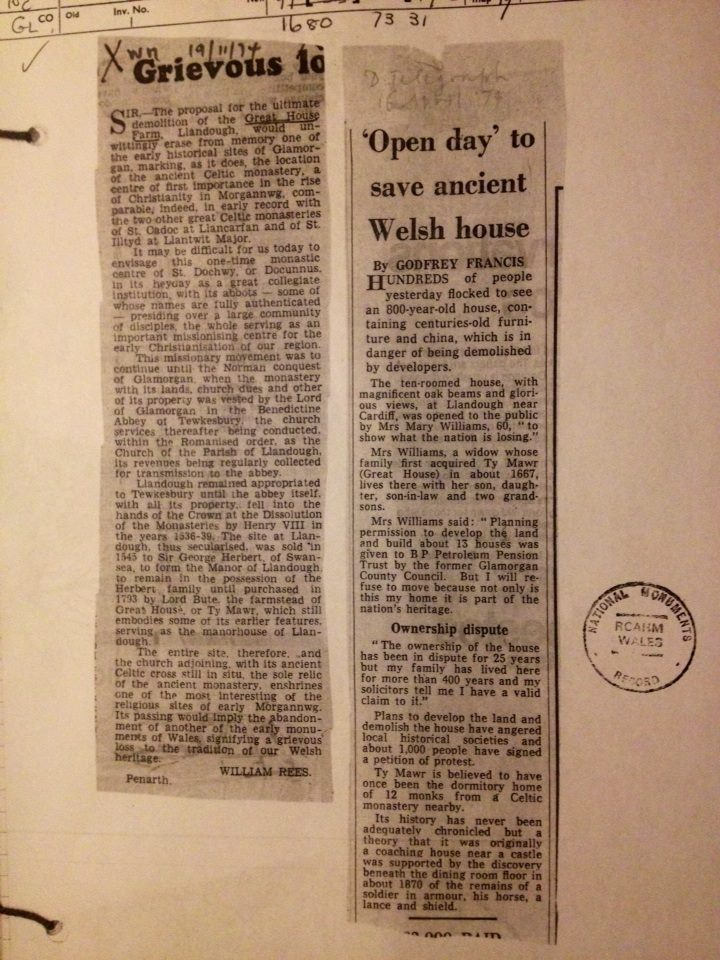
\includegraphics[width=0.85\textwidth]{newspaper_open_day.jpg}
    \caption{``Open Day to Save Ancient Welsh House'' --- South Wales Echo, 1974}
    \label{fig:open-day}
\end{figure}

\newpage

\subsection{Article 2: ``Chainsaw Farmer Vows to Fight On''}

\begin{newspaperquote}
\textbf{Source:} South Wales Echo\\
\textbf{Date:} 1988 (exact date unknown)\\
\textbf{Headline:} ``Chainsaw Farmer Vows to Fight On''\\
\textbf{Byline:} Andrew Penman
\end{newspaperquote}

\textbf{Article Text:}

\begin{quote}
A FARMER who beat-off bailiffs with a chainsaw last night vowed to continue his defiant fight for his Cardiff home.

``I am here to stay and I will fight this to the death,'' said Mr Bill Buckler after the four-hour showdown.

Yesterday's events began when five bailiffs and around 15 police officers arrived at Great House Farm, Llandough.

Mr Buckler blocked the narrow drive with a tractor, locked the farmhouse doors and barred windows.

``They smashed the lock on the gate and walked round the tractor,'' Mr Buckler said.

``Then they started smashing the doors with poleaxes. My children were right behind the door when the axe came through.

``That's when I started my chainsaw and pushed it through the door. They backed off then.''

His distressed wife, Branwen, left the farm with the couple's children, aged two, three and four. Mr Buckler and several friends and tenants remained.

The scenes were the latest episode in a battle between the Buckler family and BP Properties.

Mr Buckler said the farm has been in the family for nearly 400 years, and remains adamant he is the owner, despite a court ruling in favour of BP Properties.

He said BP had no claim over the farm except for what they had obtained through the courts.

``They have got no documents for it. If it's theirs, why have I never paid a penny in rent for it in my life?''

A farm tenant claimed the latest flare-up was brought about by the Cardiff Bay development.

``This land would be worth a fortune,'' said Mr Christopher Thompson.

``Luxury houses could be built up here to overlook Cardiff Bay. The rich would get richer and the poor poorer.''

A spokesman for BP PLC in London said the ``unpleasant'' events at the farm were regretted. He could not say if or when the bailiffs might return.

He claimed the farm was owned by BP Properties, which allowed Mr Buckler's late mother to live in it rent-free because of her ill health.

``When Mrs Buckler died in 1983 it became clear her son was not going to leave,'' said the spokesman.

``We looked at the problem, which was a sticky one, and in May 1984 we started court proceedings.''

Mr Buckler lost the court hearing in Cardiff and did not appeal.

A South Wales Police spokesman emphasised the officers at the scene were present to prevent a breach of the peace, and not to assist bailiffs.
\end{quote}

\vspace{0.5cm}
\begin{figure}[H]
    \centering
    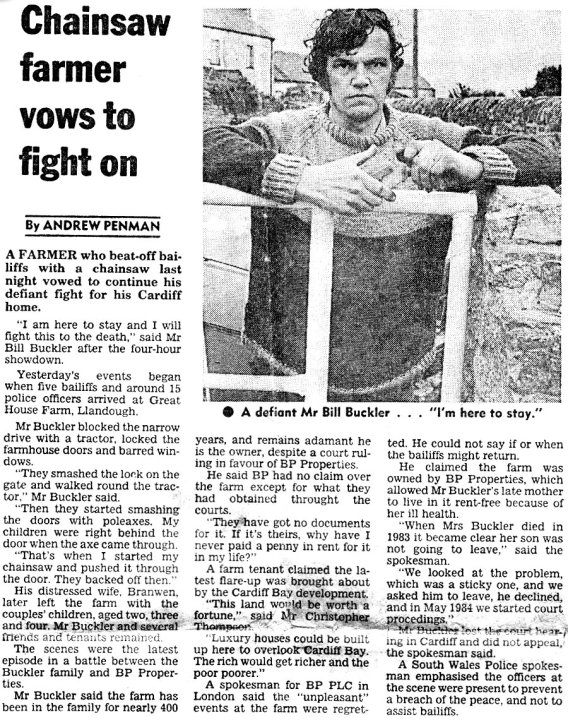
\includegraphics[width=0.85\textwidth]{newspaper_chainsaw_vows.jpg}
    \caption{``Chainsaw Farmer Vows to Fight On'' --- South Wales Echo, 1988}
    \label{fig:chainsaw-vows}
\end{figure}

\newpage

\subsection{Article 3: Police Standoff at Great House Farm}

\begin{newspaperquote}
\textbf{Source:} Unknown Newspaper\\
\textbf{Date:} 1988\\
\textbf{Caption:} ``Police wait outside the farmhouse during the four-hour showdown yesterday.''
\end{newspaperquote}

\begin{figure}[H]
    \centering
    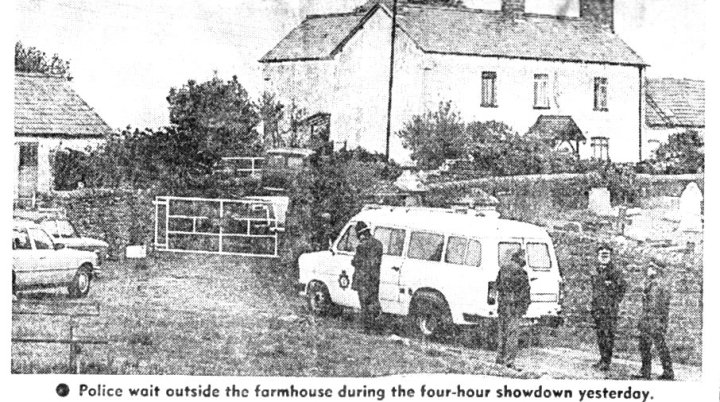
\includegraphics[width=0.9\textwidth]{newspaper_police_showdown.jpg}
    \caption{Police wait outside Great House Farm during the four-hour standoff}
    \label{fig:police-showdown}
\end{figure}

\textit{This photograph shows the police presence during the standoff at Great House Farm. Note the farmhouse in the background, which would be demolished shortly after this photograph was taken.}

\newpage

\subsection{Article 4: ``History Fight to Save Farm''}

\begin{newspaperquote}
\textbf{Source:} South Wales Echo\\
\textbf{Date:} December 3, 1988\\
\textbf{Headline:} ``History Fight to Save Farm''\\
\textbf{Byline:} Peter Bibby
\end{newspaperquote}

\textbf{Article Text:}

\begin{quote}
THE threatened farmhouse at the centre of an eviction row will be visited by historic buildings inspectors this weekend to see if it is worth saving from demolition.

Officials from the Welsh historic monuments body, Cadw, confirmed today they are considering an appeal to ask the Secretary of State for Wales to protect Great House Farm, Llandough, near Cardiff, as a listed building.

The family of farmer Billy Buckler, evicted from the farmhouse by BP bailiffs earlier this week, called in Cadw in a last-ditch bid to save their old home.

Mr Buckler's family have been fighting a 33-year legal battle to prove they own the old farmhouse, parts of which could date back to the 12th Century.

\textbf{Injunction}

But after Law Lords appeal judges ruled in favour of BP Properties this year, the bailiffs moved in. Mr Buckler, a 39-year-old father of three, has been in Llandough Hospital since his eviction on Wednesday.

BP said they intend to demolish the farmhouse and outbuildings on the 10-acre site overlooking Cardiff Bay and put in for planning permission to build new homes.

The family claim that within hours of forcing their way in to their house, the bailiffs had begun the demolition work and a High Court judge issued an interim injunction ordering that the farmhouse and its contents must not be touched.

A spokeswoman for Cadw confirmed they were considering ``spot-listing'' the farmhouse, an emergency procedure in which any building which may be of architectural or historical importance can be protected.

She said: ``An inspector has been taken off another case to look at this and we are trying to move as quickly as possible.''

\textbf{Razed}

``He will be paying a visit to the farmhouse, look at any records of the history of the area and discuss it with the Royal Commission for Ancient and Historical Monuments.''

But Cadw may have acted fast. On Monday the High Court are to consider the case for saving Great House Farm, and if the Bucklers fail to have the order extended, the farmhouse could be razed to the ground within days.
\end{quote}

\vspace{0.5cm}
\begin{figure}[H]
    \centering
    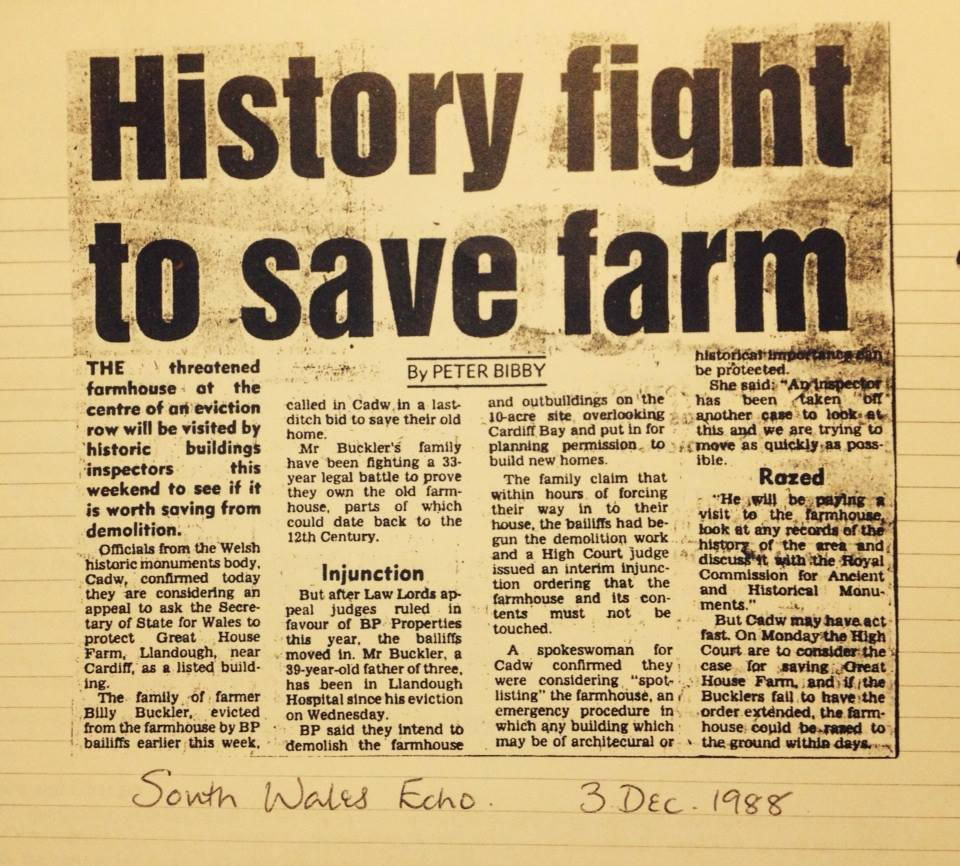
\includegraphics[width=0.85\textwidth]{newspaper_history_fight.jpg}
    \caption{``History Fight to Save Farm'' --- South Wales Echo, December 3, 1988}
    \label{fig:history-fight}
\end{figure}

\newpage

\subsection{Article 5: ``Farmer Fails in Final Eviction Hearing''}

\begin{newspaperquote}
\textbf{Source:} Western Mail\\
\textbf{Date:} December 6, 1988\\
\textbf{Headline:} ``Farmer Fails in Final Eviction Hearing''
\end{newspaperquote}

\textbf{Article Text:}

\begin{quote}
A FAMILY'S long and bitter battle for an historic farmhouse in Llandough appeared to be over last night after a High Court decision went against them and the Welsh historic monuments organisation decided to take no further action.

Farmer Billy Buckler and his wife, Branwen, had been hoping to hang on to the reputedly 800-year-old Great House Farm at Llandough and its prime 10-acre estate overlooking Cardiff Bay so that the question of ownership could be decided by the European Court.

\textbf{Destroying}

But after a hearing in chambers a judge at Cardiff Crown Court dismissed an application by Mr and Mrs Buckler for an injunction to restrain BP Properties Ltd, the owners of the land, from destroying or damaging the fabric of the building.

Their solicitor, Mr Colin Jongman, said after the hearing, ``There are no more steps that can be taken now that the building can be knocked down.''

He added that if the building was knocked down, there was little point seeking a declaration from the European Court that they could occupy the building.

A spokesperson there told the Western Mail the house was not of sufficient architectural merit and the land on which it stands was not of sufficient archaeological interest.

Following the court hearing, Mrs Janet Harris, Mr Buckler's sister, said the house had been in the family for four generations.

``It is reputed to be 800 years old and yet it seems they can destroy it on what is a whim.''

She forecast that ``they will have it down as fast as they can now'' and said their only hope was that Cadw would accept it as a listed building.

Judge Norman Francis giving his judgment in open court said that after the Buckler's unsuccessfully sought leave to appeal to the House of Lords against an Appeal Committee ruling they had exhausted the remedies available to them under the laws of England and Wales.

Their case was that there was a triable issue for the Court of Human Rights to consider and that the status quo as to the building and fittings should be preserved until it had been decided.

\textbf{Relief}

The judge said there seemed doubt whether the plaintiffs had acted in time for the European Commission to consider the case.

The fact that somebody chooses at the eleventh hour to apply to the Commission could not set up a right to ``injunctive relief.'' It would be novel for a court in this country to grant an injunction to hold up the effects of a judgment until the Court of Human Rights should rule on it, said the judge.

The battle for the farmhouse and estate has been waged for 33 years by the Buckler family.
\end{quote}

\vspace{0.5cm}
\begin{figure}[H]
    \centering
    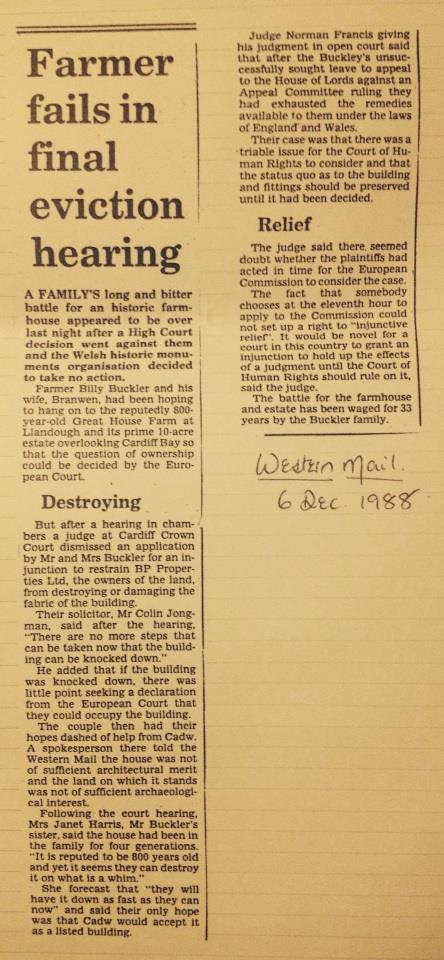
\includegraphics[width=0.85\textwidth]{newspaper_farmer_fails.jpg}
    \caption{``Farmer Fails in Final Eviction Hearing'' --- Western Mail, December 6, 1988}
    \label{fig:farmer-fails}
\end{figure}

\newpage

\subsection{Article 6: ``Tears Flow as 800 Year-Old Farm House is Razed at Last''}

\begin{newspaperquote}
\textbf{Source:} Unknown Newspaper\\
\textbf{Date:} December 1988\\
\textbf{Headline:} ``Tears Flow as 800 Year-Old Farm House is Razed at Last''
\end{newspaperquote}

\textbf{Article Text:}

\begin{quote}
THE FINAL chapter in the 35-year battle over the ownership of Great House Farm in Llandough ended early yesterday when a team moved in to demolish the 800-year-old farmhouse.

The twenty-strong team moved in with bulldozers just after 4am and by breakfast time there was not a building left standing on the ten-acre site which overlooks Cardiff Bay.

The demolition was watched by farmer's wife Branwen Buckler and her three children who wept as their family home was flattened by a bulldozer just one day after possession had been granted to the owners, BP Properties Ltd.

A High Court ruled that William and Branwen Buckler had no right to remain in the house. Mr Buckler, who admitted not paying rent for 35 years, had claimed he had the rights to the house. But a High Court judge on Monday rejected an appeal to extend an injunction to prevent the house from being demolished.

And that was the end of the legal fight for the Bucklers who had even taken their fight to keep their home where their family have lived for 400 years, to the House of Lords.

Speaking after the demolition of her home Mrs Buckler said that she and her family were ``absolutely devastated'' by the events of the previous 24 hours.

``Great House Farm was more than just a house. It was the family history with all the people who have been born or died there over the last 400 years. It is irreplaceable,'' she explained.

``Now we are left with no home, no plans, no income and no Christmas. My young son has asked me how Father Christmas is going to come down the chimney if it has been knocked down.''
\end{quote}

\vspace{0.5cm}
\begin{figure}[H]
    \centering
    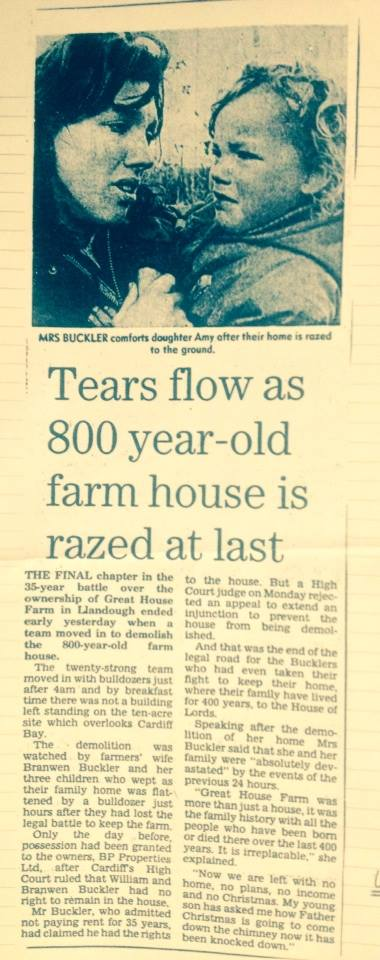
\includegraphics[width=0.75\textwidth]{newspaper_tears_flow.jpg}
    \caption{``Tears Flow as 800 Year-Old Farm House is Razed at Last'' --- December 1988}
    \label{fig:tears-flow}
\end{figure}

\newpage

\subsection{Article 7: ``Billy's Unhappy Family''}

\begin{newspaperquote}
\textbf{Source:} South Wales Echo\\
\textbf{Date:} Saturday, December 3, 1988\\
\textbf{Headline:} ``Billy's Unhappy Family''\\
\textbf{Byline:} Jim Clarke
\end{newspaperquote}

\textbf{Article Text:}

\begin{quote}
WHEN the bailiffs refused to let South Wales farmer Billy Buckler back into his family home they found eight other people sharing the rambling old farmhouse.

What were they all doing there? It seems that Billy Buckler has his family, his friends and then his friends' friends and then friends of friends turned up.

By JIM CLARKE

at Great House Farm in Llandough, Cardiff, for short stays that become permanent residences.

So the eviction of Billy, his wife Branwen and their three children Hywel, Rhys and Amy has made another group of people being made homeless.

Some of the tenants are unemployed and had the rent of the farm paid by the Vale of Glamorgan Borough Council.

One man works in a Cardiff club and two others will have to abandon business projects as a result of the eviction.

``Billy and Branwen have had a hard time of it recently, but we're all tried to get behind them and help get the farm back on its feet,'' said Chris Thompson.

Thirty-year-old Chris had just started a light haulage business backed by the Enterprise Allowance Scheme.

``It was going really well and I had plenty of work coming in, but without a base to work from or a phone I've had it,'' he said.

The bailiffs refused to comment on the allegations by the former tenants.

Karen Griffiths, aged 21, from Cardiff, told how the pressure of the legal battles with BP had taken their toll on Billy.

``Sometimes we've seen him break down and cry.''

Most of the nine people who were evicted had been living a semi-communal life at the farm for around a year.

Karen, who was made redundant from Llandaff Tech earlier this year, and her friend Terry Rayment had been travelling and living on a bus for a time before they found a place to stay at the farm --- now they are back on the bus in a nearby lay-by with their two dogs, a cat and all the possessions they could carry out of the farm.

``The farm was a happy place to stay,'' said Terry, who has known the family for years.

Karen told how the residents of Great House Farm would go out on ``wood runs'' together, collecting fuel from the nearby woods to feed the open fires in the huge farmhouse.
\end{quote}

\vspace{0.5cm}
\begin{figure}[H]
    \centering
    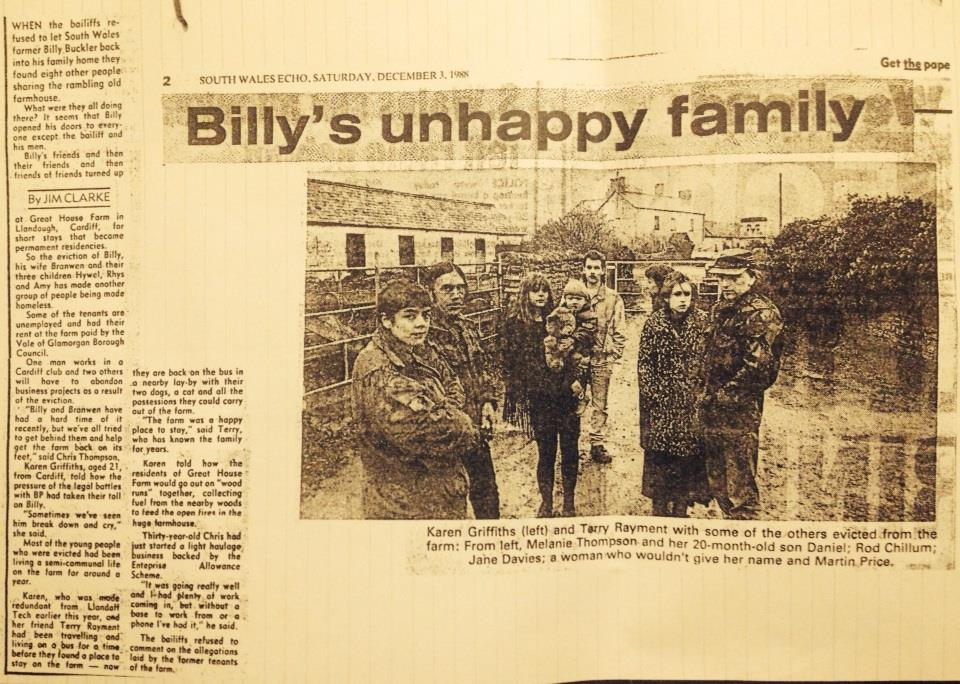
\includegraphics[width=0.85\textwidth]{newspaper_billys_family.jpg}
    \caption{``Billy's Unhappy Family'' --- South Wales Echo, December 3, 1988}
    \label{fig:billys-family}
\end{figure}

\newpage

\subsection{Article 8: ``From Farm to a Bus''}

\begin{newspaperquote}
\textbf{Source:} South Wales Echo\\
\textbf{Date:} 1989\\
\textbf{Headline:} ``From Farm to a Bus''\\
\textbf{Byline:} Peter Collins
\end{newspaperquote}

\textbf{Article Text:}

\begin{quote}
SOUTH Wales farmer Billy Buckler, whose home was demolished last year after a 40-year-old row over ownership, now plans to live in an old bus which he is converting into a mobile home.

Until December last year Mr Buckler and his family lived at Great House Farm, Llandough. But following a High Court hearing, BP Properties, the owners of the land, moved in and demolished the property.

Since then Mr Buckler, his wife, Branwen, and their three children have been living with his sister in Penarth.

``Now I've got to start from scratch again,'' said Mr Buckler. ``I have three children and my wife is expecting a baby. My sister cannot be expected to put up with that.

``I shall just have to start from scratch. They have taken everything from me and my family. I have lost my livelihood.''

Mr Buckler claimed that £30,000 worth of his personal possessions had been taken from the Great House Farm site following the demolition.
\end{quote}

\vspace{0.5cm}
\begin{figure}[H]
    \centering
    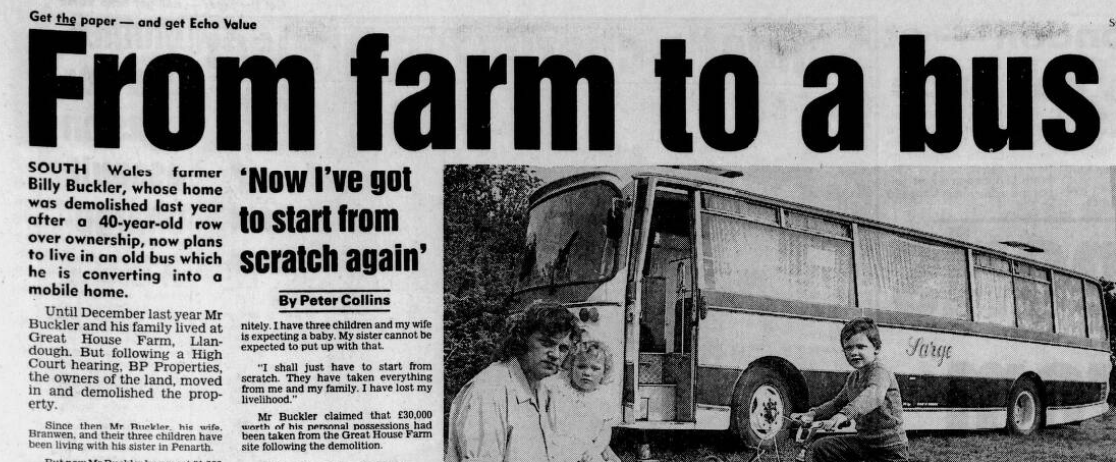
\includegraphics[width=0.85\textwidth]{newspaper_farm_to_bus.png}
    \caption{``From Farm to a Bus'' --- South Wales Echo, 1989}
    \label{fig:farm-to-bus}
\end{figure}

\newpage

\subsection{Article 9: ``Charge Against Evicted Farmer Dropped''}

\begin{newspaperquote}
\textbf{Source:} South Wales Echo\\
\textbf{Date:} 1989 (exact date unknown)\\
\textbf{Headline:} ``Charge Against Evicted Farmer Dropped''
\end{newspaperquote}

\textbf{Article Text:}

\begin{quote}
AN ALLEGATION that South Wales farmer Billy Buckler used threatening words and behaviour at his former home last year was withdrawn by the Crown Prosecution Service at Barry magistrates court yesterday.

Buckler, who lived at Great House Farm, Llandough, until it was demolished by the owners, BP Properties, in November last year, was alleged to have committed the offence in Llandough on April 29.

Mr Jeff Clarke, prosecuting, told the court that the summons was now legally ``out of time'' and could not proceed. He was therefore withdrawing it.

Buckler is due to appear in court again on February 3 to face charges of assault and wanton and furious driving at Great House Farm in November, last year.

He is currently living at an address in Penarth and has been ordered by the court not to go within half a mile of the Great House Farm site.
\end{quote}

\vspace{0.5cm}
\begin{figure}[H]
    \centering
    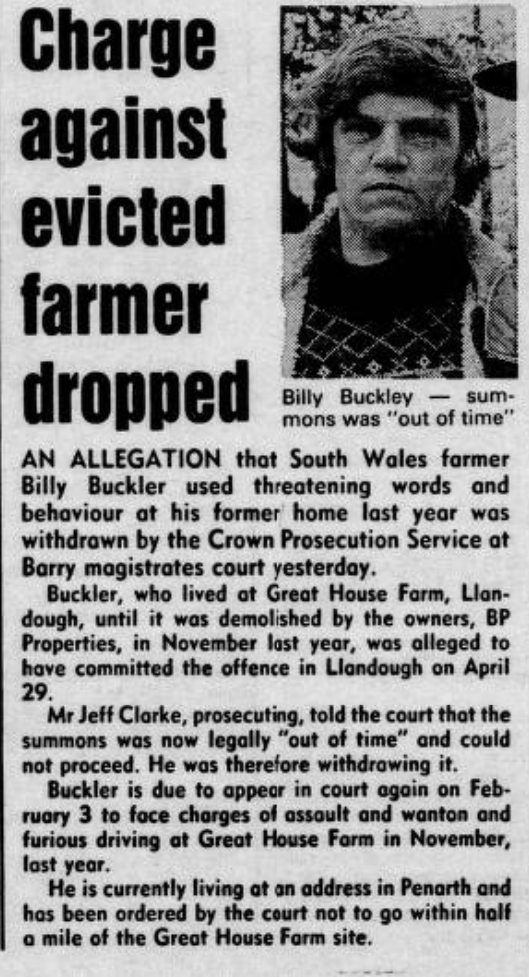
\includegraphics[width=0.85\textwidth]{newspaper_charge_dropped.png}
    \caption{``Charge Against Evicted Farmer Dropped'' --- South Wales Echo, 1989}
    \label{fig:charge-dropped}
\end{figure}

\newpage

\subsection{Additional Press References}

The following additional newspaper articles have been identified through archive searches:

\begin{enumerate}[label=\arabic*.]
    \item \textbf{``Evicted farmer refusing medical attention''} --- South Wales Echo, Saturday 30 April 1988
    
    \textit{Excerpt:} ``...check-up But Mr Buckler is refusing to leave the Great House Farm at Llandough near Cardiff for medical attention because he fears the bailiffs will return. A dozen police officers were on the farm as the bailiffs tried to evict the Buckler family...''
    
    \item \textbf{``Evicted farmer freed after pleading guilty''} --- South Wales Echo, Thursday 23 March 1989
    
    \textit{Excerpt:} ``...A FARMER who lost his family home at Great House Farm Llandough when the premises were demolished at the end of last year today admitted two...''
    
    \item \textbf{``Buckler freed on bail''} --- South Wales Echo, Saturday 10 December 1988
    
    \textit{Excerpt:} ``...Buckler aged 40 who lived with family at Great House Farm Llandough until was demolished by BP Properties this week was freed on bail by magistrates yesterday...''
    
    \item \textbf{``Harm charge farmer freed''} --- South Wales Echo, Friday 24 March 1989
    
    \textit{Excerpt:} ``...'I will fight on to the death' FARMER BILLY Buckler vowed to continue his fight over the loss of his historic family home and more than 70 acres of land...''
    
    \item \textbf{``All I've got left''} --- South Wales Echo, Tuesday 13 December 1988
    
    \textit{Excerpt:} ``...who lived at Great House Farm Llandough near Cardiff said: ``All I've got left are the clothes stand up in'' Mr Buckler evicted from the farmhouse by BP Properties who demolished the building a week later said:...''
\end{enumerate}

\newpage

% The 1987 Court Case: BP Properties Ltd v Buckler
\section{The 1987 Court Case: BP Properties Ltd v Buckler}

\subsection{The Legal Issue}

The case concerned a dispute over possession of Great House Farm. William Buckler junior claimed a possessory title by adverse possession by himself and his parents before him.

\subsection{The Court's Finding}

The Court of Appeal (Dillon LJ) held:

\begin{enumerate}[label=\arabic*.]
    \item The suggested possessory title was not made out for Great House Farm as a whole
    \item However, for the farmhouse and garden, there was no doubt that Mr. Buckler junior had exclusive possession, as his parents did before him, and no rent had been paid since 1953
    \item Mrs. Buckler's license to occupy the farmhouse and garden rent-free granted by BP Properties Ltd did not extinguish her adverse possession because it was granted by the wrong company --- it should have been granted by BP Pension Trust Ltd, the legal owner
\end{enumerate}

\subsection{The Contradiction}

\begin{grievance}
The judge stated that Mrs. Buckler's reply to BP Pension Trust Ltd didn't count because BP Properties Ltd and BP Pension Trust Ltd were two separate companies. However, in William Buckler's subsequent appeal, he argued that BP Pension Trust should have been the claimant. The judge dismissed the appeal, citing that both BP companies were ``effectively the same.''

This creates a fundamental contradiction: the family allegedly lost because Mrs. Buckler didn't reply (to the ``right'' company), yet both companies were considered the same entity when it suited the court's reasoning.
\end{grievance}

\newpage

% The Marconi Connection: A Suppressed History?
\section{The Marconi Connection: A Suppressed History?}

\subsection{The First Radio Transmission Over Open Sea}

\begin{keyfact}
On May 13, 1897, Guglielmo Marconi made telecommunications history by transmitting a radio signal across open sea for the first time. The transmission was from Lavernock Point, near Penarth, to Flat Holm Island in the Bristol Channel --- a distance of 3 miles (4.8 km).
\end{keyfact}

The message sent in Morse code was: \textbf{``Are you ready''}

The reply from George Kemp: \textbf{``YES LOUD AND CLEAR''}

\subsection{Marconi's Connection to Great House Farm}

According to family history and the blog ``The Great House Farm Story'':

\begin{timeline}
\textbf{May 1897} --- At age 22, Guglielmo Marconi slept at Great House Farm in a four-poster bed while working on his wireless telegraphy experiments. The Williams family (Buckler ancestors) reportedly rode Marconi and his equipment by horse and cart to Lavernock Point to conduct his famous experiments.
\end{timeline}

The family also sold a dining table in the 1970s that was said to have been used by Marconi during his experiments.

\subsection{The Cardiff Bay Sculpture Controversy}

\begin{keyfact}
In 2024, a four-meter-tall sculpture was installed on Cardiff Bay Barrage to celebrate Cardiff's history and connection to Flat Holm Island. The sculpture depicts a radio transmitter tower warping into an old-fashioned analogue radio set.
\end{keyfact}

\subsubsection{The Deliberate Omission}

\begin{grievance}
A full review of the sculpture plans took place in 2022. It was decided that there would be \textbf{no mention of Marconi} on the sculpture due to his historical links to the regime of Benito Mussolini, as well as links to fascism and antisemitism.

Cardiff Council stated: ``The council in no way condones Marconi's links to fascism and antisemitism.''
\end{grievance}

\newpage

% The 1994 Archaeological Excavation
\section{The 1994 Archaeological Excavation}

\subsection{Discovery and Excavation}

\begin{timeline}
\textbf{March 1994} --- Cotswold Archaeological Trust (now Cotswold Archaeology) was commissioned to undertake an excavation at the former site of Great House Farm. The excavation was sponsored by Ideal Homes Ltd (now part of Persimmon Homes).
\end{timeline}

The excavation revealed one of the most significant archaeological sites in Wales:

\begin{keyfact}
\textbf{1,026 burials} were investigated, making this the largest early Christian cemetery excavated to date in Wales. The excavation covered an area of 0.22 hectares.
\end{keyfact}

\subsection{Key Archaeological Findings}

\subsubsection{The Cemetery}

\begin{itemize}
    \item \textbf{814 inhumations} were excavated and recorded
    \item \textbf{212 disarticulated bone groups} were identified
    \item The cemetery dated from the late Iron Age through to the early medieval period
    \item Three distinct areas were identified within the cemetery
    \item Infant burials (approximately 700) represented the latest phase of burial activity
\end{itemize}

\subsubsection{The Roman Villa}

Evidence confirmed:
\begin{itemize}
    \item A substantial Roman villa with stone foundations
    \item At least five rooms or passages
    \item A hypocaust system (underfloor heating)
    \item The villa was enclosed by a well-built wall with twin parallel ditches
    \item A bath complex with a well-preserved cold plunge bath
\end{itemize}

\newpage

% Legal Analysis
\section{Legal Analysis}

\subsection{The Doctrine of Adverse Possession}

Adverse possession is a legal doctrine that allows a person to claim ownership of land by occupying it for a specified period without the legal owner's permission, provided certain conditions are met.

\subsubsection{Requirements for Adverse Possession}

Under English and Welsh law, the requirements are:

\begin{enumerate}[label=\arabic*.]
    \item \textbf{Factual Possession}: The claimant must have exclusive physical control of the land
    \item \textbf{Intention to Possess (Animus Possidendi)}: The claimant must demonstrate an intention to possess the land as their own
    \item \textbf{Without Permission}: The possession must be without the owner's consent
    \item \textbf{Continuous Period}: For unregistered land, 12 years under the Limitation Act 1980
\end{enumerate}

\subsection{The BP Properties Ltd v Buckler Precedent}

The case established an important principle in adverse possession law:

\begin{keyfact}
\textbf{Principle}: Where a license is offered but never refused, this may be taken to mean that the license has been granted. A unilateral license can stop time running for adverse possession.
\end{keyfact}

Dillon LJ stated: ``So far as Mrs. Buckler was concerned, even though she did not `accept' the terms of the letters, BP Properties Ltd would, in the absence of any repudiation by her of the two letters, have been bound to treat her as in possession as licensee on the terms of the letters.''

\newpage

% Paths to Justice and Compensation
\section{Paths to Justice and Compensation}

\subsection{Strategic Overview}

\begin{tcolorbox}[colback=blue!5,colframe=darkblue,title=\textbf{Strategic Reality}]
Courts alone = slow, expensive, uncertain

Pressure + Law combined = money

Your strongest leverage is moral clarity + documentary timeline, not technical rent law.
\end{tcolorbox}

\subsection{Path 1: Civil Claim (Historical Wrong / Misfeasance)}

\begin{action}
\textbf{Target}: Corporate successors (BP entities, developers, ground rent companies)

\textbf{Basis}: Abuse of power, unlawful eviction, unjust enrichment

\textbf{Remedy}: Damages + interest

\textbf{Status}: TO BE INITIATED
\end{action}

\subsection{Path 2: Human Rights Claim}

\begin{action}
\textbf{Use}: ECHR principles (even if time-barred domestically)

\textbf{Aim}: Pressure, declarations of wrongdoing, leverage for settlement

\textbf{Key Rights}:
\begin{itemize}
    \item Article 8: Right to respect for private and family life, home
    \item Article 1 of Protocol 1: Protection of property
    \item Article 6: Right to a fair trial
\end{itemize}

\textbf{Status}: TO BE INITIATED
\end{action}

\subsection{Path 3: Public Inquiry / Ombudsman Route}

\begin{action}
\textbf{Frame as}: Systemic abuse of tenants by estate and energy interests

\textbf{Goal}: Official finding $\rightarrow$ compensation scheme or ex gratia payment

\textbf{Potential Avenues}:
\begin{itemize}
    \item Welsh Government Petitions Committee
    \item UK Parliament Early Day Motion
    \item Local Government Ombudsman
    \item Parliamentary Ombudsman
\end{itemize}

\textbf{Status}: TO BE INITIATED
\end{action}

\subsection{Path 4: Restitution / Profits-Based Claim}

\begin{action}
\textbf{Argument}: Land value uplift directly flowed from unlawful dispossession

\textbf{Remedy}: Account of profits (hard but powerful)

\textbf{Calculation Factors}:
\begin{itemize}
    \item Current value of the developed land
    \item Value of the farm at time of dispossession
    \item Profits made by developers (Ideal Homes/Persimmon)
    \item Archaeological value of artifacts recovered
\end{itemize}

\textbf{Status}: TO BE INITIATED
\end{action}

\subsection{Path 5: Media and Parliamentary Strategy}

\begin{action}
\textbf{Key Narratives}:
\begin{itemize}
    \item Hospital removal without charges
    \item Demolition while family barred from returning
    \item 400+ years of occupation ended by corporate interests
    \item Possible Marconi connection suppressed
    \item Archaeological treasures taken without compensation
\end{itemize}

\textbf{Goal}: Force corporate settlement to avoid reputational damage

\textbf{Status}: TO BE INITIATED
\end{action}

\newpage

% Action Plan and Roadmap
\section{Action Plan and Roadmap}

\subsection{Phase 1: Documentation and Evidence Gathering (Months 1--3)}

\begin{action}
\textbf{Immediate Actions}:
\begin{enumerate}[label=\arabic*.]
    \item \textbf{Obtain Court Records}:
    \begin{itemize}
        \item Full transcript of BP Properties Ltd v Buckler (1987)
        \item All possession order documents from 1955, 1962, 1974
        \item Any appeal documentation
    \end{itemize}
    
    \item \textbf{Freedom of Information Requests}:
    \begin{itemize}
        \item Ministry of Justice: BP vs Buckler case files
        \item Cardiff Council: Planning records for Great House Farm site
        \item National Museum of Wales: Location of artifacts from 1994 excavation
        \item Welsh Government: Any records relating to the case
    \end{itemize}
    
    \item \textbf{Newspaper Archive Research}:
    \begin{itemize}
        \item 1974 press coverage of the case
        \item Reports of the 1987 case
        \item Articles about the demolition
        \item Any mention of Marconi connection to the farm
    \end{itemize}
    
    \item \textbf{Family Documentation}:
    \begin{itemize}
        \item Compile all family photographs of the farm
        \item Record oral histories from surviving family members
        \item Document any remaining correspondence
        \item Create family tree showing continuous occupation
    \end{itemize}
\end{enumerate}
\end{action}

\subsection{Phase 2: Legal Research and Strategy (Months 2--4)}

\begin{action}
\textbf{Legal Actions}:
\begin{enumerate}[label=\arabic*.]
    \item \textbf{Engage Specialist Solicitors}:
    \begin{itemize}
        \item Firms specializing in land law and historical claims
        \item Human rights specialists
        \item Consider conditional fee arrangements
    \end{itemize}
    
    \item \textbf{Research Precedents}:
    \begin{itemize}
        \item Other successful historical land injustice claims
        \item ECHR cases on property rights
        \item Unjust enrichment cases against corporations
    \end{itemize}
    
    \item \textbf{Corporate Investigation}:
    \begin{itemize}
        \item Current status of BP Properties Ltd
        \item Successor liability of BP Pension Trust
        \item Current ownership of the developed land
    \end{itemize}
\end{enumerate}
\end{action}

\subsection{Phase 3: Public Awareness Campaign (Months 3--6)}

\begin{action}
\textbf{Media and Public Actions}:
\begin{enumerate}[label=\arabic*.]
    \item \textbf{Create Website}: Document the full story with evidence
    \item \textbf{Social Media Campaign}: Share the story on relevant platforms
    \item \textbf{Contact Journalists}: Target investigative journalists and Welsh media
    \item \textbf{Parliamentary Engagement}:
    \begin{itemize}
        \item Contact local MP and MS (Member of Senedd)
        \item Submit petition to Welsh Parliament
        \item Request Early Day Motion in UK Parliament
    \end{itemize}
\end{enumerate}
\end{action}

\subsection{Phase 4: Formal Legal Action (Months 6--12)}

\begin{action}
\textbf{Legal Proceedings}:
\begin{enumerate}[label=\arabic*.]
    \item \textbf{Letter Before Action}: To corporate successors
    \item \textbf{Ombudsman Complaint}: If applicable
    \item \textbf{Court Proceedings}: If settlement not reached
    \item \textbf{ECHR Application}: If domestic remedies exhausted
\end{enumerate}
\end{action}

\newpage

% Conclusion
\section{Conclusion}

The Buckler family's case represents more than a simple land dispute. It embodies centuries of Welsh history, from Roman villas to medieval monasteries, from agricultural tenancies to corporate land grabs. The family's 400-year occupation of Great House Farm was ended not by any criminal wrongdoing, but by a combination of legal technicalities, corporate power, and what appears to be systematic pressure tactics.

\subsection{The Case for Justice}

The evidence supports the following conclusions:

\begin{enumerate}[label=\arabic*.]
    \item The Buckler family had a legitimate claim to Great House Farm based on:
    \begin{itemize}
        \item Over 400 years of continuous occupation
        \item An equitable title agreement with Daniel Thomas
        \item The theft of deeds that prevented proof of ownership
    \end{itemize}
    
    \item The legal process was flawed:
    \begin{itemize}
        \item Contradictory reasoning about the two BP companies
        \item Disproportionate enforcement measures
        \item Use of detention without criminal charges
    \end{itemize}
    
    \item The family's suffering was extreme:
    \begin{itemize}
        \item Denial of basic utilities (water)
        \item Physical removal from hospital
        \item Destruction of their home and belongings
        \item Prevention from retrieving personal effects
    \end{itemize}
    
    \item Corporate beneficiaries profited:
    \begin{itemize}
        \item BP entities gained valuable development land
        \item Developers (Ideal Homes/Persimmon) profited from housing development
        \item The Crown/museums may have gained archaeological treasures
    \end{itemize}
\end{enumerate}

\subsection{A Call to Action}

\begin{tcolorbox}[colback=gold!10,colframe=gold!70!black,title=\textbf{The Buckler Family's Request}]
\begin{enumerate}[label=\arabic*.]
    \item \textbf{Justice}: Acknowledgment of the wrongs committed against the family
    \item \textbf{Compensation}: Financial restitution for the loss of home, livelihood, and heritage
    \item \textbf{Recognition}: Public acknowledgment of the family's historical connection to the land
    \item \textbf{Return}: Of any artifacts or treasures excavated from beneath the farm
    \item \textbf{Remembrance}: A memorial or plaque at the site commemorating the family's 400+ years of occupation
\end{enumerate}
\end{tcolorbox}

\vspace{1cm}

\begin{center}
\rule{0.6\textwidth}{0.5pt}\\[0.5cm]
{\large\itshape ``Justice will not be served until those who are unaffected\\
are as outraged as those who are.''}\\[0.3cm]
--- Benjamin Franklin
\end{center}

\newpage

% Appendices
\appendix

\section{Key Legal Documents}

\subsection{BP Properties Ltd v Buckler [1987] EWCA Civ 2}

Citation: (1988) 55 P \& CR 337; [1987] 2 EGLR 168

Court: Court of Appeal (Civil Division)

Judges: Dillon LJ, Balcombe LJ

\subsection{Key Excerpt from Dillon LJ's Judgment}

``As BP Properties is not obliged by the same constraints as the Pension Trust and since we wish to help you as much as possible, we are prepared to allow you to remain in occupation of the house and garden rent free for as long as you may wish and for the rest of your life if you so desire.''

``So far as Mrs. Buckler was concerned, even though she did not `accept' the terms of the letters, BP Properties Ltd would, in the absence of any repudiation by her of the two letters, have been bound to treat her as in possession as licensee on the terms of the letters. They could not have evicted her (if they could have done so at all) without determining the licence.''

``I can see no escape therefore from the conclusion that, whether she liked it or not, from the time of her receipt of the letters, Mrs Buckler was in possession of the farmhouse and garden by the licence of BP Properties Ltd, and her possession was no longer adverse.''

\section{Sources and References}

\subsection{Legal Sources}

\begin{enumerate}[label={[\arabic*]}]
    \item BP Properties Ltd v Buckler [1987] EWCA Civ 2; (1988) 55 P \& CR 337
    \item Limitation Act 1980
    \item Land Registration Act 2002
    \item Agricultural Holdings Act 1948
\end{enumerate}

\subsection{Newspaper Archive Sources}

\begin{enumerate}[label={[\arabic*]}]
    \item ``Open Day to Save Ancient Welsh House'', South Wales Echo, 1974 (Godfrey Francis)
    \item ``Chainsaw Farmer Vows to Fight On'', South Wales Echo, 1988 (Andrew Penman)
    \item ``History Fight to Save Farm'', South Wales Echo, December 3, 1988 (Peter Bibby)
    \item ``Farmer Fails in Final Eviction Hearing'', Western Mail, December 6, 1988
    \item ``Tears Flow as 800 Year-Old Farm House is Razed at Last'', December 1988
    \item ``Billy's Unhappy Family'', South Wales Echo, December 3, 1988 (Jim Clarke)
    \item ``From Farm to a Bus'', South Wales Echo, 1989 (Peter Collins)
    \item ``Charge Against Evicted Farmer Dropped'', South Wales Echo, 1989
\end{enumerate}

\subsection{Historical Sources}

\begin{enumerate}[label={[\arabic*]}]
    \item Thomas, A. and Holbrook, N., \textit{Excavations at Great House Farm, Llandough, Cardiff, South Glamorgan: A Preliminary Report} (1994)
    \item Owen-John, H., `Llandough: the rescue excavation of a multi-period site near Cardiff, South Glamorgan', in Robinson, D.M. (ed.), \textit{Biglis, Callicot and Llandough: Three Late Iron Age and Romano-British Sites in South-East Wales} (BAR Brit. Ser., 188, Oxford, 1988)
    \item Loe, L., \textit{Health and socio-economic status in early medieval Wales} (PhD thesis, University of Bristol, 2004)
\end{enumerate}

\subsection{Online Sources}

\begin{enumerate}[label={[\arabic*]}]
    \item ``The Great House Farm Story'', United Technocracy blog (2012)
    \item ``Marconi: world's first radio message was sent in Wales'', Herald.Wales (2021)
    \item ``The story behind the brand new sculpture at Cardiff Bay Barrage'', WalesOnline (2024)
    \item Cotswold Archaeology, ``An Early-medieval Monastic Cemetery at Llandough'' (2011)
\end{enumerate}

\section{Contact Information}

For updates on this case and to support the Buckler family's quest for justice:

\begin{center}
\begin{tcolorbox}[colback=lightgray,colframe=darkblue,width=0.8\textwidth]
\centering
\textbf{Buckler Family Justice Campaign}\\[0.3cm]
This document is a living record.\\
Updates will be added as the case progresses.
\end{tcolorbox}
\end{center}

\end{document}
